\documentclass[letterpaper,12pt]{article}
\usepackage{tabularx} % extra features for tabular environment
\usepackage{amsmath}  % improve math presentation

\usepackage{amssymb}

\usepackage{witharrows}
\usepackage{graphicx} % takes care of graphic including machinery
\usepackage[margin=1in,letterpaper]{geometry} % decreases margins
\usepackage{cite} % takes care of citations
\usepackage[final]{hyperref} % adds hyper links inside the generated pdf file
\hypersetup{
	colorlinks=true,       % false: boxed links; true: colored links
	linkcolor=blue,        % color of internal links
	citecolor=blue,        % color of links to bibliography
	filecolor=magenta,     % color of file links
	urlcolor=blue         
}
\usepackage{blindtext}
%++++++++++++++++++++++++++++++++++++++++


\begin{document}

\title{Enter the Op-Amp}
\author{Dev Patel}
\date{\today}
\maketitle


In this short paper I'll dive into Op-Amp Basics. This paper is intended as a supplement to the TJHSST Electronics club presentation on Op-Amps. Please reach out to tjhsstmicroelect@gmail.com for any questions about the Club, TJHSST Electronics course offerings, or Electronics Senior Research.


\section{What is an Op-Amp?}

An Op-Amp is short term for Operational Amplifier. An Operational Amplifier can serve many purposes, and is most commonly used to amplify a signal. In our audio chain project, we will use the Op-Amp to amplify the signal coming from a microphone. 

Op-Amps are most commonly used for the following:
\begin{itemize}
  \item Signal Conditioning
  \item Adding, Subtracting, Multiplying, or Dividing a Signal
\end{itemize}

At the most fundamental level, an Op-Amp has 3 ports. One non-inverting input, One inverting input, and one output port. The inverting input and the non-inverting input of the Op-Amp respectively invert and don't invert the signal. For example, if we were to feed a sine wave \begin{math}(sin{theta}\end{math} into our non-inverting input, and had a voltage gain of 1, the output function would be \begin{math}(-sin{theta}\end{math}. Don't worry if you don't know what all of those terms mean, we are going to dive into them in the next subsection.

\subsection{Differential Amplifier}
The Op-Amps we will be using for our project are called Differential Amplifiers. These Differential Amps use a dual supply (+V, and -V). The dual supply ensures a constant supply of voltage. While we won't dive deep into the inner circuitry of a Differential Amp, they generally use forward biased transistors to balance the output current. Ideally, when no signal is input into the amp, these transistors would ensure that no signal comes out of the amp. However, in the real world, small amounts of signal noise may pass through. The Op-Amp has two input terminals - the inverting and non-inverting terminal. The Op-Amp will only respond to the difference between the two terminals. That's why if you are only using 1 terminal, it is important to ground the other terminal, otherwise the Op-Amp will not read the difference between the Voltages, and it won't respond with the correct output voltage.

An important concept in Op-Amps is impedance. Input impedance is the ratio of input voltage to input current. Op-Amps do not like any current that enter the circuit, and try to close it out completely. In an ideal circuit, we assume input impedance to be infinity. Input impedance exists in the real world however, it's negligible. Output impedance is the amount of resistance inside the Op-Amp. The Op-Amp is assumed to be a perfect voltage source, so the ideal value is 0. However, in the real world, small amounts of resistance are present in the Amp.

An Ideal Op-Amp has an open loop gain of infinity. However, in the real world, these gains usually start a certain value (like 40dB), and they follow a frequency response curve.

\begin{figure}
    \centering
    \includegraphics[width=100mm,scale=1]{bob1.png}
    \caption{An example Open-Loop Frequency response curve of an Op-Amp. Taken from electronics-tutorials.ws}
\end{figure}

An example of this frequency response curve is shown in Figure 1. At the -3db point, this Op-Amp begins to follow a linear path. We can represent the slope of this curve as the Voltage Gain times the Frequency Bandwidth.

We can calculate the voltage gain of any op-amp with the Voltage Gain Formula
\begin{equation}
   V_g = \frac{V_o}{V_i}
   \label{Eq:VoltageGain} %the label lets you refer to the equation later
\end{equation}

\section{ Op-Amps In Action}

In this section we will explore Inverting and Non-Inverting Amplifier configurations with a trusty LM741. The LM741, a Texas Instruments device, is the holy grail of Op-Amps for beginners. It's robust, relatively quick, and can handle almost whatever you throw at it. Let's take a look at some of the LM741's characteristics. All of the following images have been taken from the LM741 Datasheet.
\begin{figure}
    \centering
    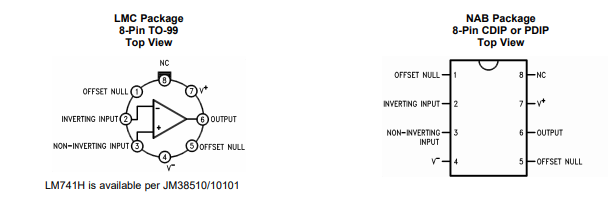
\includegraphics[width=150mm,scale=1]{op-amp.PNG}
    \caption{Taken from LM741 Datasheet}
\end{figure}
Looking closely at Figure 2, we can see that our LM741 has 8 pins. We aren't going to focus on the offset null pins, or pin 8, so we only really have 5 pins to worry about. Pin 2 and 3 are our input pins, 4 and 7 handle our constant power, and pin 6 is our output. Now that we know this, we can start drawing up some circuitry. It's important to remember while in theory an Op-Amp has infinite gain, in the real world signal noise and current limitations make massive gains off a single amp unlikely. For the LM741, our recommended maximum gain is around 10.

\subsection{Inverting Op-Amp Configuration}
The Inverting Op-Amp (as the name implies) inverts and amplifies the signal in. In Figure 3, we can see what a sample inverting Op-Amp configuration looks like.
\begin{figure}
    \centering
    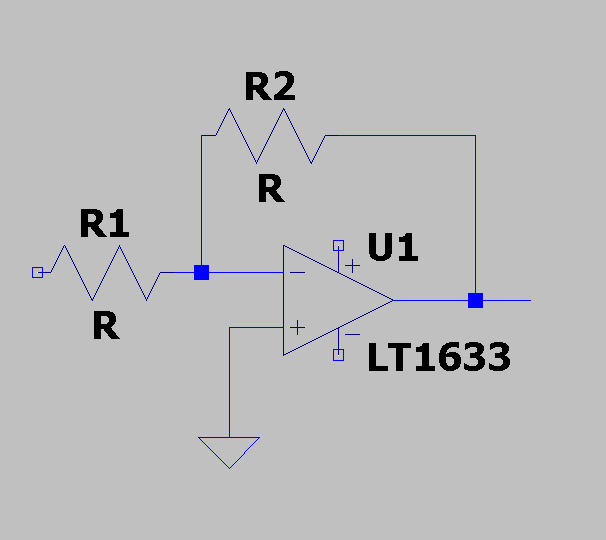
\includegraphics[scale=0.5]{op-amp2.PNG}
    \caption{LTSpice example Op-Amp Config}
\end{figure}
In Figure 3, we use an LT633 Op-Amp, but the general configuration for all Inverting Op-Amps is the same. Signal in enters through the negative port (the path with R1 in the figure). In an inverting Op-Amp, the voltage gain can be calculated by using the following expression:
\begin{equation}
   \frac{-R_1}{R_2}
   \label{Eq:Inverting} %the label lets you refer to the equation later
\end{equation}
This expression multiplied by Vin will give you the voltage coming out of the Op-Amp. One important thing to note about Op-Amps is often there is a current drop after you amplify. This current drop will become an issue later in our audio chain project as we reach the Speaker Stage.

\subsection{Non-Inverting Op-Amp Configuration}
The Non-Inverting Op-Amp (as the name implies) only amplifies the signal in. In Figure 4, we can see what a sample non-inverting Op-Amp configuration looks like.
\begin{figure}
    \centering
    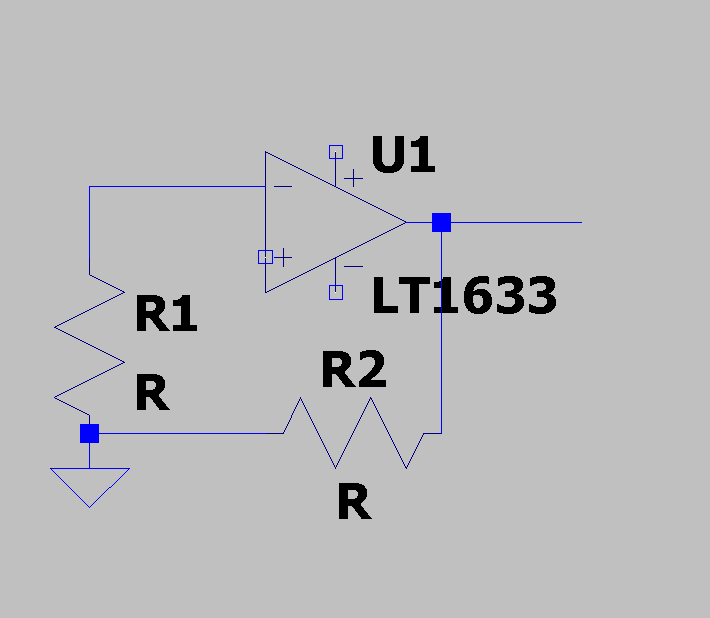
\includegraphics[scale=0.5]{op-amp3.PNG}
    \caption{LTSpice example Op-Amp Config}
\end{figure}
In Figure 4, we use an LT633 Op-Amp, but the general configuration for all Non-Inverting Op-Amps is the same. Signal in enters through the positive port (left empty in the figure). In a non-inverting Op-Amp, the voltage gain can be calculated by using the following expression:
\begin{equation}
   1+\frac{R_1}{R_2}
   \label{Eq:Non-Inverting} %the label lets you refer to the equation later
\end{equation}
This expression multiplied by Vin will give you the voltage coming out of the Op-Amp. 
\section{Conclusions}
This has been a brief overview of Op-Amps. Now go and create your own Op-Amp Circuits!
\end{document}
